\section{The \gls{fdtd}}\label{sec:fdtd}
The goal of this section is to outline the basics of numerical sound field simulation by using the \gls{fdtd} method. The principles this kind of numerical simulation will be described, so that the method can be adapted to investigate the behaviour of one or more loudspeakers in a sound field. 
The approach of \gls{fdtd} is to solve the wave equation by a finite-difference approximation for both time and space derivatives. This makes it possible to easily simulate the sound pressure and particle velocity of a speaker at any time step. 
%One advantage of using \gls{fdtd} is that the impulse response of a specific loudspeaker can be incorporated into the simulation and therefore it is possible to simulate the speaker that is used in this project. 
For using \gls{fdtd} with a specific loudspeaker, all simulations have to be done in a relatively narrow frequency band, in order for the simulation to give a good approximation to the real world behaviour. An \gls{fdtd} cannot cover the whole human hearing range accurately. The scope of the semester project is a frequency range from \SIrange{60}{300}{\hertz}. An important property of \gls{fdtd}-simulations is, that the calculations are performed in time domain, which means, that the pressure and the particle velocity at any specified time step can be analyzed directly by solving two coupled equations.\citep{fdtddaga}. This section will end out with a \gls{fdtd} model of a 3 dimensional space.\\

\subsection{\gls{fdtd} wave equation}
In \gls{fdtd}-simulation, there typically are two equations, which need to be solved. When simulating a sound field, the first formula is the Euler \autoref{fdtd_euler}, which describes the relation between the gradient of the pressure $p$ and the derivative of the particle velocity $\vec{v}$ with respect to time. 

\begin{equation}\label{fdtd_euler}
\frac{\partial \vec{v}}{\partial t} =- \frac{1}{\rho}\vec{\triangledown }p
\end{equation}

    \startexplain
    	\explain{$\rho$ is the density of the medium }{\si{\kilo\gram\per\cubic\meter}}
        \explain{$\partial t$ is an infinitesimal time step}{\si{\second}}
        \explain{$p$ is the pressure }{\si{\pascal}}
        \explain{$\vec{v}$ is the particle velocity}{\si{\meter\per\second}}
    \stopexplain

\autoref{fdtd_euler} is only valid with small variation in pressure. The second \autoref{fdtd_linear} is the linear continuity equation. The equation describes the relation between the derivative of the pressure $p$ with respect of time and the velocity gradient $\triangledown\vec{v}$. They are related through the density of the medium and the speed of sound. 

 \begin{equation}\label{fdtd_linear}
\frac{\partial p}{\partial t} =- \rho c^2 \vec{\triangledown }\vec{v}
\end{equation}

    \startexplain
    	\explain{$\rho$ is the density of the medium }{\si{\kilo\gram\per\cubic\meter}}
        \explain{$\partial t$ is an infinitesimal time step}{\si{\second}}
        \explain{$p$ is the pressure }{\si{\pascal}}
        \explain{$c$ is the speed of sound }{\si{\meter\per\second}}
        \explain{$\vec{v}$ is the particle velocity}{\si{\meter\per\second}}
    \stopexplain

By use of the derivation, both equations are approximated linearly at every point in a three dimensional cartesian grid. This is done with discrete time steps.
%Both equations are approximated by using finite difference for every point in space and time, by using a 3 dimensional grid of the space. 


\subsection{\gls{fdtd} using Cartesian grid}

Using a Cartesian grid for \gls{fdtd} approximation is a well known technique (see \citep{finiteproblems}) and will also be employed in this project. The Cartesian grid is set up using the sound pressure \autoref{fdtd_linear} and the particle velocity \autoref{fdtd_linear} as the unknown quantities, which have to be solved for in every point in space.  A small grid is visualized in \autoref{fig:fdtd_cartesian_grid}

\begin{figure}[H]
	\centering
\begin{picture}(0,0)%
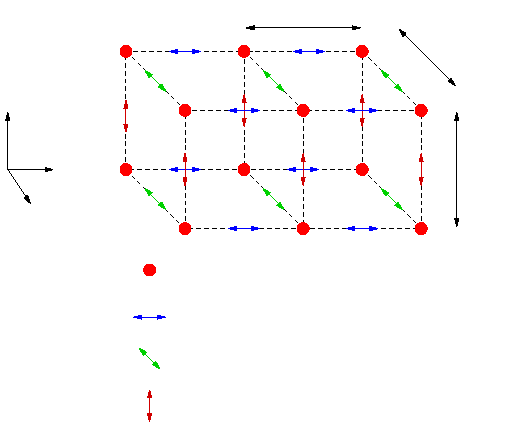
\includegraphics{fdtd_grid.pdf}%
\end{picture}%
\setlength{\unitlength}{4144sp}%
%
\begingroup\makeatletter\ifx\SetFigFont\undefined%
\gdef\SetFigFont#1#2#3#4#5{%
  \reset@font\fontsize{#1}{#2pt}%
  \fontfamily{#3}\fontseries{#4}\fontshape{#5}%
  \selectfont}%
\fi\endgroup%
\begin{picture}(3869,3327)(3541,-1288)
\put(6841,1649){$\delta y$}%
\put(3556,1244){$z$}%
\put(4006,704){$x$}%
\put(3826,344){$y$}%
\put(5806,1874){$\delta x$}%
\put(4996,-61){Pressure point}%
\put(4996,-421){Particle velocity x-direction}%
\put(4996,-781){Particle velocity y-direction}%
\put(4996,-1096){Particle velocity z-direction}%
\put(7066,704){$\delta z$}%
\end{picture}%
	\caption{A 3 dimensional example of a Cartesian grid.}
		\label{fig:fdtd_cartesian_grid}
\end{figure}


The grid points are built of positions that are described as $(i\,\delta x,j\,\delta y,k\,\delta z)$ at a time $t=[l]\delta t$. The time step is visualized in \autoref{fig:fdtd_transient_point}.

\begin{figure}[H]
	\centering
\begin{picture}(0,0)%
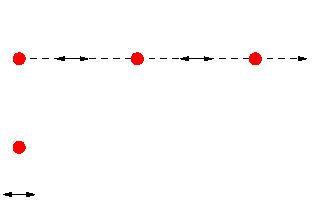
\includegraphics{fdtd_transient_point.pdf}%
\end{picture}%
\setlength{\unitlength}{4144sp}%
%
\begingroup\makeatletter\ifx\SetFigFont\undefined%
\gdef\SetFigFont#1#2#3#4#5{%
  \reset@font\fontsize{#1}{#2pt}%
  \fontfamily{#3}\fontseries{#4}\fontshape{#5}%
  \selectfont}%
\fi\endgroup%
\begin{picture}(2518,1594)(4804,-854)
\put(5266,-421){Pressure point}%
\put(5266,-781){Particle velocity}%
\put(5076,469){$[l-\frac{1}{2}] \delta t$}%
\put(5671, 29){$[l] \delta t$}%
\put(6456, 29){$[l+1]\delta t$}%
\put(5961,469){$[l+\frac{1}{2}]\delta t$}%
\put(7246,254){$t$}%
\end{picture}%
	\caption{Transient definition points of sound $p$ pressure and particle velocity $\vec{v}$}
		\label{fig:fdtd_transient_point}
\end{figure}

$\delta x,\delta y,\delta z$ are the spatial discretization steps as shown in \autoref{fig:fdtd_cartesian_grid} and $\delta t$ is the time spatial discretization step as shown in \autoref{fig:fdtd_transient_point}. $i,j,k$ are the discrete indices for the points in the grid and $l$ is the discrete time index. For every axis, the corresponding particle velocity has to be determined at a position in \autoref{fdtd_component} at an intermediate time $t=[l\pm\frac{1}{2}]$ .

\begin{equation}\label{fdtd_component}
\vec{v}= \begin{bmatrix}
v_x[(i\pm \frac{1}{2})\,\delta x,j\,\delta y,k\,\delta z]\\
v_y[i\,\delta x,(j\pm \frac{1}{2})\,\delta y,k\,\delta z]\\
v_z[i\,\delta x,j\,\delta y,(k\pm \frac{1}{2})\,\delta z]
\end{bmatrix}
\end{equation}
The pressure is determined at position $p_{(i,j,k)}^{[l+1]}$. It can be chosen to start with either pressure or velocity arbitrarily. The time step $\delta t$ can be regarded as a scaling factor for time, because Python only works with integer indices. This means $\delta t$ is implemented in the formulas and not in the iteration step. The time $\pm \frac{1}{2}$ is also changed to a integer with adding $\frac{1}{2}$. This scalar is only relevant in the implementation and is disregarded in the rest of this section. The same applies for the step sizes $\delta x$, $\delta y$ and $\delta z$.\\


Solving for $(v_x)_{(i+\frac{1}{2},j,k)}^{[l+\frac{1}{2}]}$ leads to following three Equations \ref{fdtd_particle_velocity}:


\begin{subequations}\label{fdtd_particle_velocity}
\begin{alignat}{2}
(v_x)_{(i+\frac{1}{2},j,k)}^{[l+\frac{1}{2}]}&= (v_x)_{(i+\frac{1}{2},j,k)}^{[l-\frac{1}{2}]}-\frac{\delta t}{\rho_0 \delta x} \left( p_{(i+1,j,k)}^{[l]} -p_{(i,j,k)}^{[l]}  \right)\\
(v_y)_{(i,j+\frac{1}{2},k)}^{[l+\frac{1}{2}]}&= (v_y)_{(i,j+\frac{1}{2},k)}^{[l-\frac{1}{2}]}-\frac{\delta t}{\rho_0 \delta y} \left( p_{(i,j+1,k)}^{[l]} -p_{(i,j,k)}^{[l]}  \right)\\
(v_z)_{(i,j,k+\frac{1}{2})}^{[l+\frac{1}{2}]}&= (v_z)_{(i,j,k+\frac{1}{2})}^{[l-\frac{1}{2}]}-\frac{\delta t}{\rho_0 \delta z} \left( p_{(i,j,k+1)}^{[l]} -p_{(i,j,k)}^{[l]}  \right)
\end{alignat}
\end{subequations}
\\



Solving for $p_{(i,j,k)}^{[l+1]}$ leads to  \autoref{fdtd_pressure}.




\begin{multline}\label{fdtd_pressure}
p_{(i,j,k)}^{[l+1]} = p_{(i,j,k)}^{[l]} - \rho_0 c^2 \delta t \Biggl( \frac{(v_x)_{(i+\frac{1}{2},j,k)}^{[l+\frac{1}{2}]} - (v_x)_{(i-\frac{1}{2},j,k)}^{[l+\frac{1}{2}]}}{\delta x} \\ 
+ \frac{(v_y)_{(i,j+\frac{1}{2},k)}^{[l+\frac{1}{2}]}-(v_y)_{(i,j-\frac{1}{2},k)}^{[l+\frac{1}{2}]}}{\delta y} +  \frac{(v_z)_{(i,j,k+\frac{1}{2})}^{[l+\frac{1}{2}]}-(v_z)_{(i,j,k-\frac{1}{2})}^{[l+\frac{1}{2}]}}{\delta z} \Biggr)
\end{multline}

\subsection{\gls{fdtd} grid boundary conditions}        
The meaning of boundary conditions in the given context is the behaviour of the simulation near and at the boundary surfaces (walls), that occur at the ends of the grid. The sound waves react differently on the walls opposed to propagation in free field conditions. Walls will act like either a reflecting surface, an absorbing surface or both. This boundary behaviour from the wall is described as an frequency dependent impedance. It is necessary to analyse and implement this in the simulation because the sound field will show a different behaviour compared to sound field without any boundaries. Within this project, the frequency dependent boundary conditions will only be a good approximation and not accurately represent free field conditions. An accurate frequency dependent model would require heavy calculations with convolution at each boundary point and at each time step \citep{finiteproblems}. This kind of calculation has a high time consumption and therefore an approximation will be used. \\
The approximation in this project will be based on the impedance approach (see \citep{FDTDmodelling}) as described above. The impedance approach can be used when walls is present in simulation and does not contain a perfect matched layer. Therefore the impedance approach can not be used for free field simulation unless the simulation is stopped just before the wave hits the boundary. Because of the way the pressure spreads along the grid, the stopped simulation will lead to some areas, typically every corner, to which the wave has not yet spread. This results in a circular shape on the simulation grid if the sound sources are placed in the middle. In this project a large room is used and the simulation will be stopped just before the boundary to simulate free field condition. Afterwards the data are cropped such that only simulating data within the area to which the sound had already spread are used. \\

The  impedance approach is usable at low frequency, meaning in a frequency range, in which the sound sources behave approximately omnidirectional \citep{FDTDmodelling}. Two kinds of absorbing boundaries are common in real life and therefore also in simulation. These boundaries are as follows:

\begin{figure}[H]
	\centering
\begin{picture}(0,0)%
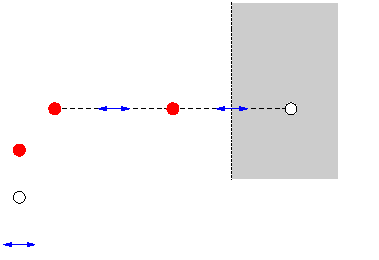
\includegraphics{fdtd_wall_reflection.pdf}%
\end{picture}%
\setlength{\unitlength}{4144sp}%
%
\begingroup\makeatletter\ifx\SetFigFont\undefined%
\gdef\SetFigFont#1#2#3#4#5{%
  \reset@font\fontsize{#1}{#2pt}%
  \fontfamily{#3}\fontseries{#4}\fontshape{#5}%
  \selectfont}%
\fi\endgroup%
\begin{picture}(2876,1975)(4534,-854)
\put(4996,-61){Pressure point}%
\put(4996,-781){Particle velocity x-direction}%
\put(4996,-421){Unknown pressure point}%
\end{picture}%
	\caption{The figure visualized a boundary plan through particle velocity plan $x$ in 1 dimension.}
		\label{fig:fdtd_boundary_pressure}
\end{figure}

For solving the problem visualized in \autoref{fig:fdtd_boundary_pressure}, an asymmetric finite-difference approximation for the space derivative is used  \citep{finiteproblems}. \autoref{fdtd_boundary_absorbing} shows the asymmetric finite-difference approximation.

\begin{equation}\label{fdtd_boundary_absorbing_velocity}
\frac{\partial p}{\partial x}\mid _{(i_0+\frac{1}{2},j,k)}^{[l]} = \frac{2}{\delta x} \left( p_{(i_0+\frac{1}{2},j,k)}^{[l]}-p_{(i_0,j,k)}^{[l]} \right)
\end{equation}\\

The advantage of \autoref{fdtd_boundary_absorbing_velocity} is that it only requires knowledge of one nearest pressure point, but it is only valid within $\delta x$.  Using the same procedure as in \autoref{fdtd_particle_velocity} just with plugging in \autoref{fdtd_boundary_absorbing_velocity} instead, the particle velocity at the boundary is approximated as \autoref{fdtd_boundary_eqp}

\begin{equation}\label{fdtd_boundary_eqp}
(v_x)_{(i_0+\frac{1}{2},j,k)}^{[l+\frac{1}{2}]}= (v_x)_{(i_0+\frac{1}{2},j,k)}^{[l-\frac{1}{2}]}-\frac{2 \delta t}{\rho_0 \delta x} \Biggl( 
p_{(i_0+\frac{1}{2},j,k)}^{[l]} -p_{(i_0,j,k)}^{[l]}  \Biggr)
\end{equation}

The only unknown in \autoref{fdtd_boundary_eqp} is $p_{(i_0+\frac{1}{2},j,k)}^{[l]}$, but it can be found by using \autoref{fdtd_boundary_absorbing}, where $v_n$ is changed with $(v_x)_{(i_0+\frac{1}{2},j,k)}^{[l]}$ and becomes \autoref{fdtd_boundary_velocity}.


\begin{multline}\label{fdtd_boundary_velocity}
(v_x)_{(i_0+\frac{1}{2},j,k)}^{[l+\frac{1}{2}]}= (v_x)_{(i_0+\frac{1}{2},j,k)}^{[l-\frac{1}{2}]}-\frac{2 \delta t}{\rho_0 \delta x} \Biggl( 
 Z_0(v_x)_{(i_0+\frac{1}{2},j,k)}^{[l]} \\
 +Z_1 \frac{\partial (v_x)_{(i_0+\frac{1}{2},j,k)}^{[l]}}{\partial t} +Z_{-1} \int_{-\infty}^{t} (v_x)_{(i_0+\frac{1}{2},j,k)}^{[l]}(\tau)d\tau -p_{(i_0,j,k)}^{[l]}
\Biggr)
\end{multline}

The integral in the \autoref{fdtd_boundary_velocity} is replaced with a sum from minus infinity to $l$ in \autoref{fdtd_boundary_velocity2}.

\begin{multline}\label{fdtd_boundary_velocity2}
(v_x)_{(i_0+\frac{1}{2},j,k)}^{[l+\frac{1}{2}]}= (v_x)_{(i_0+\frac{1}{2},j,k)}^{[l-\frac{1}{2}]}-\frac{2 \delta t}{\rho_0 \delta x} \Biggl( 
 Z_0(v_x)_{(i_0+\frac{1}{2},j,k)}^{[l]} \\
+Z_1\frac{(v_x)_{(i+\frac{1}{2},j,k)}^{[l+\frac{1}{2}]}-(v_x)_{(i+\frac{1}{2},j,k)}^{[l-\frac{1}{2}]}}{\delta t}+Z_{-1} \delta t \sum_{m=-\infty}^{l} \left( (v_x)_{(i+\frac{1}{2},j,k)}^{[m+\frac{1}{2}]} \right) -p_{(i,j,k)}^{[l]}
\Biggr)
\end{multline}

The last unknown variable is the particle velocity $v_x$ at time $t=[l]$. To find a solution for $v_x$ at time $t=[l]$, a linear interpolation between $v_x$ at time $t=[l \pm \frac{1}{2}]$ is used \citep{finiteproblems}. The resulting particle velocity will be expressed as \autoref{fdtd_boundary_result}

\begin{multline}\label{fdtd_boundary_result}
(v_x)_{(i_0+\frac{1}{2},j,k)}^{[l+\frac{1}{2}]}= \alpha (v_x)_{(i_0+\frac{1}{2},j,k)}^{[l-\frac{1}{2}]} + \beta \frac{2 \delta t}{\rho_0 \delta x} \Biggl( 
 Z_0(v_x)_{(i_0+\frac{1}{2},j,k)}^{[l]} \\
-Z_{-1} \delta t \sum_{m=-\infty}^{l} \left( (v_x)_{(i+\frac{1}{2},j,k)}^{[m+\frac{1}{2}]} \right) -p_{(i,j,k)}^{[l]}
\Biggr)
\end{multline}


         \startexplain
    		\explain{$\alpha = \frac{1-\frac{Z_0}{Z_{FDTD}} \frac{2Z_1}{Z_{FDTD}} \delta t}{1+\frac{Z_0}{Z_{FDTD}} \frac{2Z_1}{Z_{FDTD}} \delta t}$ }{\si{1}}
    		\explain{$\beta = \frac{1}{1-\frac{Z_0}{Z_{FDTD}} \frac{2Z_1}{Z_{FDTD}} \delta t}$ }{\si{1}}
    		\explain{$Z_{FDTD} = \frac{\rho_0 \delta x}{\delta t}$ }{\si{\newton\second\meter^{-3}}}
    \stopexplain



\subsection{\gls{fdtd} grid cell size}

The choice of grid cell size for \gls{fdtd} is a critical parameter, which must fulfill some problem specific constraint \citep{Kunz1993}. The grid cell size has to be small enough to contain data for all specified simulated frequencies, which means that the grid cell size has to be smaller than the smallest wavelength $\lambda$. As the frequency rises the wave length is decreasing. This means the grid cell size constrain is determined by the highest frequency of interest in the \gls{fdtd} simulation. Opposed to that, the grid cell size should be relatively large, in order to keep the computational power down, that is required to run the simulation. The grid cell size therefore has to be chosen intelligently, for which \citep{Kunz1993} displays a solution. After the grid cell size is chosen the Courant stability condition determines the maximum time step. The maximum time step size, which will be calculated based on the grid cell size, will be the used. A smaller time step size does not improve the accuracy in general. \\


The boundary for the smallest grid cell size is the Nyquist rate, which states that the wavelength shall at least be twice as big as the grid cell size $\delta$. Since $\delta x$, $\delta y$ and $\delta z$ have the same size only $\delta$ will be used to represent the grid step size. The Nyquist rate is the lower boundary, but since the simulation is an approximation and is not exact and the smallest wavelength is not precise, $\delta$ has to be more than two samples per wavelength. To find a optimal grid size the grid dispersion error which relates to the wave propagation speed through the grid will be taken intro account. The error occurs because the wave propagates with different slightly speeds through the grid. This error is depending on the relative direction of the wave. The grid dispersion error is propertional to the grid cell size, which means that the error is decreased with smaller $\delta$\citep{Kunz1993}. 
Often if $ \delta \leq \frac{1}{10}\lambda_{min}$ the formerly mentioned constraint is met. The solution therefore a good compromise between computation resource and approximation error. The grid cell size in this project is therefore set according to \autoref{fdtd_delta_stepsize}.

\begin{equation}\label{fdtd_delta_stepsize}
\delta x = \delta y = \delta z \leq \frac{1}{10} \frac{c}{f_{max}}
\end{equation}

    \startexplain
    	\explain{$\delta$ is the grid cell size }{\si{1}}
        \explain{$x$, $y$ and $z$ is the direction}{\si{1}}
        \explain{$c$ is the speed of sound}{\si{\meter\per\second}}
        \explain{$f_{max}$ is the maximum frequency in the simulation}{\si{\hertz}}
    \stopexplain
    
    
    

\subsection{\gls{fdtd} time step size and stability}   \label{sec:fdtd_time_stepsize} 
The time step size for \gls{fdtd} follows from the Courant condition \citep{Kunz1993}. The aim of the project is not to analyse the condition of Courant. This section will therefore only give a short overview on the most important aspects of the condition and on how to use the condition to calculate the time step size. Considering a plane wave, the Courant condition states that, in one time step, any point on the wave must not pass through more than one cell. During one time step the wave can propagate only from one cell to its nearest neighbors \citep{Kunz1993}. To determine the time step size the time step $\delta t $ can therefore be determined by the speed of sound and the grid cell size as in \autoref{fdtd_time_stepsize}.



\begin{equation}\label{fdtd_time_stepsize}
\delta t \leq \frac{1}{\sqrt{\frac{1}{(\delta x)^2}+\frac{1}{(\delta x)^2}+\frac{1}{(\delta x)^2} }\cdot c}
\end{equation}
        \startexplain
    		\explain{$\delta$ is the step size}{\si{1}}
        \explain{$t$ is the time indicator}{\si{\second}}
        \explain{$c$ is the speed of sound}{\si{\meter\per\second}}
    \stopexplain
    
Making the time step size smaller than stated by \autoref{fdtd_time_stepsize} will not improve the result, in fact the equation calculates the time step size where the grid dispersion error is minimal \citep{Kunz1993}. Unless the dispersion error is minimized, the time step might even be  smaller because of the stability condition. 
A stable simulation is only guaranteed under certain conditions. Because \autoref{fdtd_boundary_result} is applied to different conditions e.g. in corner or flat walls, a stable simulation is not possible in general, only under certain conditions which depend on time and grid cell size. It has been shown, that the simulation is stable if $Z_0$ and $Z_{1}$ are positive for all simulation regions and if \autoref{fdtd_time_stepsize_boundary} is satisfied \citep{finiteproblems}.

\begin{equation}\label{fdtd_time_stepsize_boundary}
\delta t \leq \sqrt{\frac{2}{3}}  \left( \frac{1}{\sqrt{\frac{1}{(\delta x)^2}+\frac{1}{(\delta x)^2}+\frac{1}{(\delta x)^2} }\cdot c} \right)
\end{equation}\\


If $Z_{-1}$ is nonzero the time step shall furthermore satisfy \autoref{fdtd_time_stepsize_boundary_Z_n1}

\begin{equation}\label{fdtd_time_stepsize_boundary_Z_n1}
c \delta t \leq \delta x \left(   \frac{1+\frac{2Z_1}{\rho_0 \delta x}}{1+\frac{2Z_{-1} \delta x}{\rho_0 c^2}}  \right)^{\frac{1}{2}}
\end{equation}

\subsection{\gls{fdtd} sound source}
The so called acoustical center of the loudspeaker used in the main project is about \SI{17}{\centi\meter} in the front of the speaker cabinet. It also has to be noted that the \gls{fdtd} sound source for the simulation is at the acoustical center and not at the position of the loudspeaker itself. Therefore the \gls{fdtd} sound source is modelled as a transparent source. The speaker cabinet may have a different effect when building a speaker array in the real world, but not at the position of the sound source in \gls{fdtd}. Therefore the speaker cabinet will not be incorporated into the simulation. The following section will briefly explain the three most common way of implementing sources as described in \citep{FDTDsource}. \\

There are two simple methods to implement a \gls{fdtd} sound source and one more advanced way to implement a \gls{fdtd} sound source. The simple ways of implementing at sound source are the hard- and the soft sources. The problem with implementing a hard source is, that the hard source overwrites the update step in the source point and therefore effectively scatters any incident field. This might correspond to a real scenario if the speaker cabinet was at the acoustical center and very reflective, but it is not and therefore this kind of source is not suitable in the given context. Secondly, the soft source is set up in a way, that the pressure from the source is added to the pressure source point, which means, that this source does not scatter. The problem with this method is that the actual excitation does not match the time function of the source. To make a source that acts like a hard source but does not scatter, the transparent source is used according to \citep{FDTDtransparent}. The explaining the implementation of transparent source is quite lengthy and has only little benefit for understanding the computational issues that are the subject of this mini-project. It will therefore be skipped. \\



%A transparent source is achieved by measuring the impulse response $I$ of the grid and using it in \autoref{fdtd_transparent_source}.
%
%\begin{multline}\label{fdtd_transparent_source}
%p_{(i_{s},j_{s},k_{s})}^{[l+1]}=p_{(i_{s},j_{s},k_{s})}^{[l]} - \rho_0 c^2 \delta t  \Biggl( \frac{(v_x)_{(i_{s}+\frac{1}{2},j_{s},k_{s})}^{[l+\frac{1}{2}]} - (v_x)_{(i_{s}-\frac{1}{2},j_{s},k_{s})}^{[l+\frac{1}{2}]}}{\delta x} +
% \frac{(v_y)_{(i_{s},j_{s}+\frac{1}{2},k_{s})}^{[l+\frac{1}{2}]}-(v_y)_{(i_{s},j_{s}-\frac{1}{2},k_{s})}^{[l+\frac{1}{2}]}}{\delta y} + \\ 
% \frac{(v_z)_{(i_{s},j_{s},k_{s}+\frac{1}{2})}^{[l+\frac{1}{2}]}-(v_z)_{(i_{s},j_{s},k_{s}-\frac{1}{2})}^{[l+\frac{1}{2}]}}{\delta z} \Biggr)
%+f^{l+1}-\sum_{m=0}^{l} \left( I^{l-m+1}f^m \right)
%\end{multline}
%
%        \startexplain
%        \explain{$(i_{s},j_{s},k_{s})$ are the source grid positions}{\si{1}}
%        \explain{$I$ is the impulse response of the grid}{\si{1}}
%    \stopexplain
%
%As it can be seen in \autoref{fdtd_transparent_source}, the source is implemented like a soft source but with a correction part $-\sum_{m=0}^{l} \left( I^{l-m+1}f^m \right)$. The correction part includes the impulse response of the \gls{fdtd} grid and has to be measured. To measure the impulse response of the grid, a Kronecker delta function is used as the sound source with unity gain. The Kronecker delta source emits an impulse with unity gain only at time one, and zero otherwise. The Kronecker delta source is implemented as a hard source \citep{FDTDtransparent}. \\
%
%
%The impulse response is measured at the source point. As stated before, the Kronecker source is implemented as a hard source. When measuring at the source point, it is therefore to be expected, that the measurement behaves as the Kronecker source signal that is sent out, because of the hard implementation of the source. To get around this, the measured pressure is not actually recorded from the source point, but calculated back from the particular velocity surrounding the source.
%%but it has to be noted that the impulse response is not the Kronecker delta function unless it is measured in the same point. The impulse response is the value the source pressure point should have been calculated to according to the particle velocity. But since the Kronecker delta is implemented as a hard source, the source pressure point will be overwritten by the Kronecker delta function and therefore the impulse response step have to be calculated from the nearest particle velocity.
%The impulse response measurement function is therefore described by \autoref{fdtd_transparent_source_impulse}:
%
%\begin{multline}\label{fdtd_transparent_source_impulse}
%I^{[l]}=p_{(i_{s},j_{s},k_{s})}^{[l-1]} - \rho_0 c^2 \delta t  \Biggl( \frac{(v_x)_{(i_{s}+\frac{1}{2},j_{s},k_{s})}^{[l-\frac{1}{2}]} - (v_x)_{(i_{s}-\frac{1}{2},j_{s},k_{s})}^{[l-\frac{1}{2}]}}{\delta x} +\\
% \frac{(v_y)_{(i_{s},j_{s}+\frac{1}{2},k_{s})}^{[l-\frac{1}{2}]}-(v_y)_{(i_{s},j_{s}-\frac{1}{2},k_{s})}^{[l-\frac{1}{2}]}}{\delta y} +  
% \frac{(v_z)_{(i_{s},j_{s},k_{s}+\frac{1}{2})}^{[l-\frac{1}{2}]}-(v_z)_{(i_{s},j_{s},k_{s}-\frac{1}{2})}^{[l-\frac{1}{2}]}}{\delta z} \Biggr)
%\end{multline}
%
%
%The Kronecker delta source will be placed in the middle of the grid, and there is only one Kronecker delta source. The particle velocity matrices for each dimension have therefore the following symmetrical $(v_x)_{(i_{s}-\frac{1}{2},j_{s},k_{s})}^{[l-\frac{1}{2}]} = -(v_x)_{(i_{s}+\frac{1}{2},j_{s},k_{s})}^{[l-\frac{1}{2}]}$. The impulse response measurement function can therefore be shortened to \autoref{fdtd_transparent_source_impulse_short}:
%
%\begin{equation}\label{fdtd_transparent_source_impulse_short}
%I^{[l]}=p_{(i_{s},j_{s},k_{s})}^{[l-1]} - 2\rho_0 c^2 \delta t  \Biggl( \frac{(v_x)_{(i_{s}+\frac{1}{2},j_{s},k_{s})}^{[l-\frac{1}{2}]}}{\delta x} +
% \frac{(v_y)_{(i_{s},j_{s}+\frac{1}{2},k_{s})}^{[l-\frac{1}{2}]}}{\delta y} +  
% \frac{(v_z)_{(i_{s},j_{s},k_{s}+\frac{1}{2})}^{[l-\frac{1}{2}]}}{\delta z} \Biggr)
%\end{equation}
%
%There is a stability condition that has to be satisfied in order to make the transparent source  stable in \gls{fdtd} simulation. The stability condition is \autoref{fdtd_transparent_source_impulse_stability} \citep{FDTDtransparent}. 
%
%
%\begin{equation}\label{fdtd_transparent_source_impulse_stability}
%\frac{c \delta t}{\delta d} \leq \frac{1}{\sqrt{N}}
%\end{equation}
%
%        \startexplain
%        \explain{$N$ is the number of dimensions}{\si{1}}
%        \explain{$\delta d$ is the smallest grid step of $\delta x$, $\delta y$ and $\delta z$}{\si{1}}
%    \stopexplain
%    
%    

